\documentclass{article}
\usepackage[utf8]{inputenc}
\usepackage{graphicx}

\title{Relatório de Análise do Agronegócio}
\author{GabrielMule\_RM560586}
\date{\today}

\begin{document}

\maketitle

\section{Produção Agrícola}
A análise da produção agrícola mostra um crescimento significativo na produção de grãos.

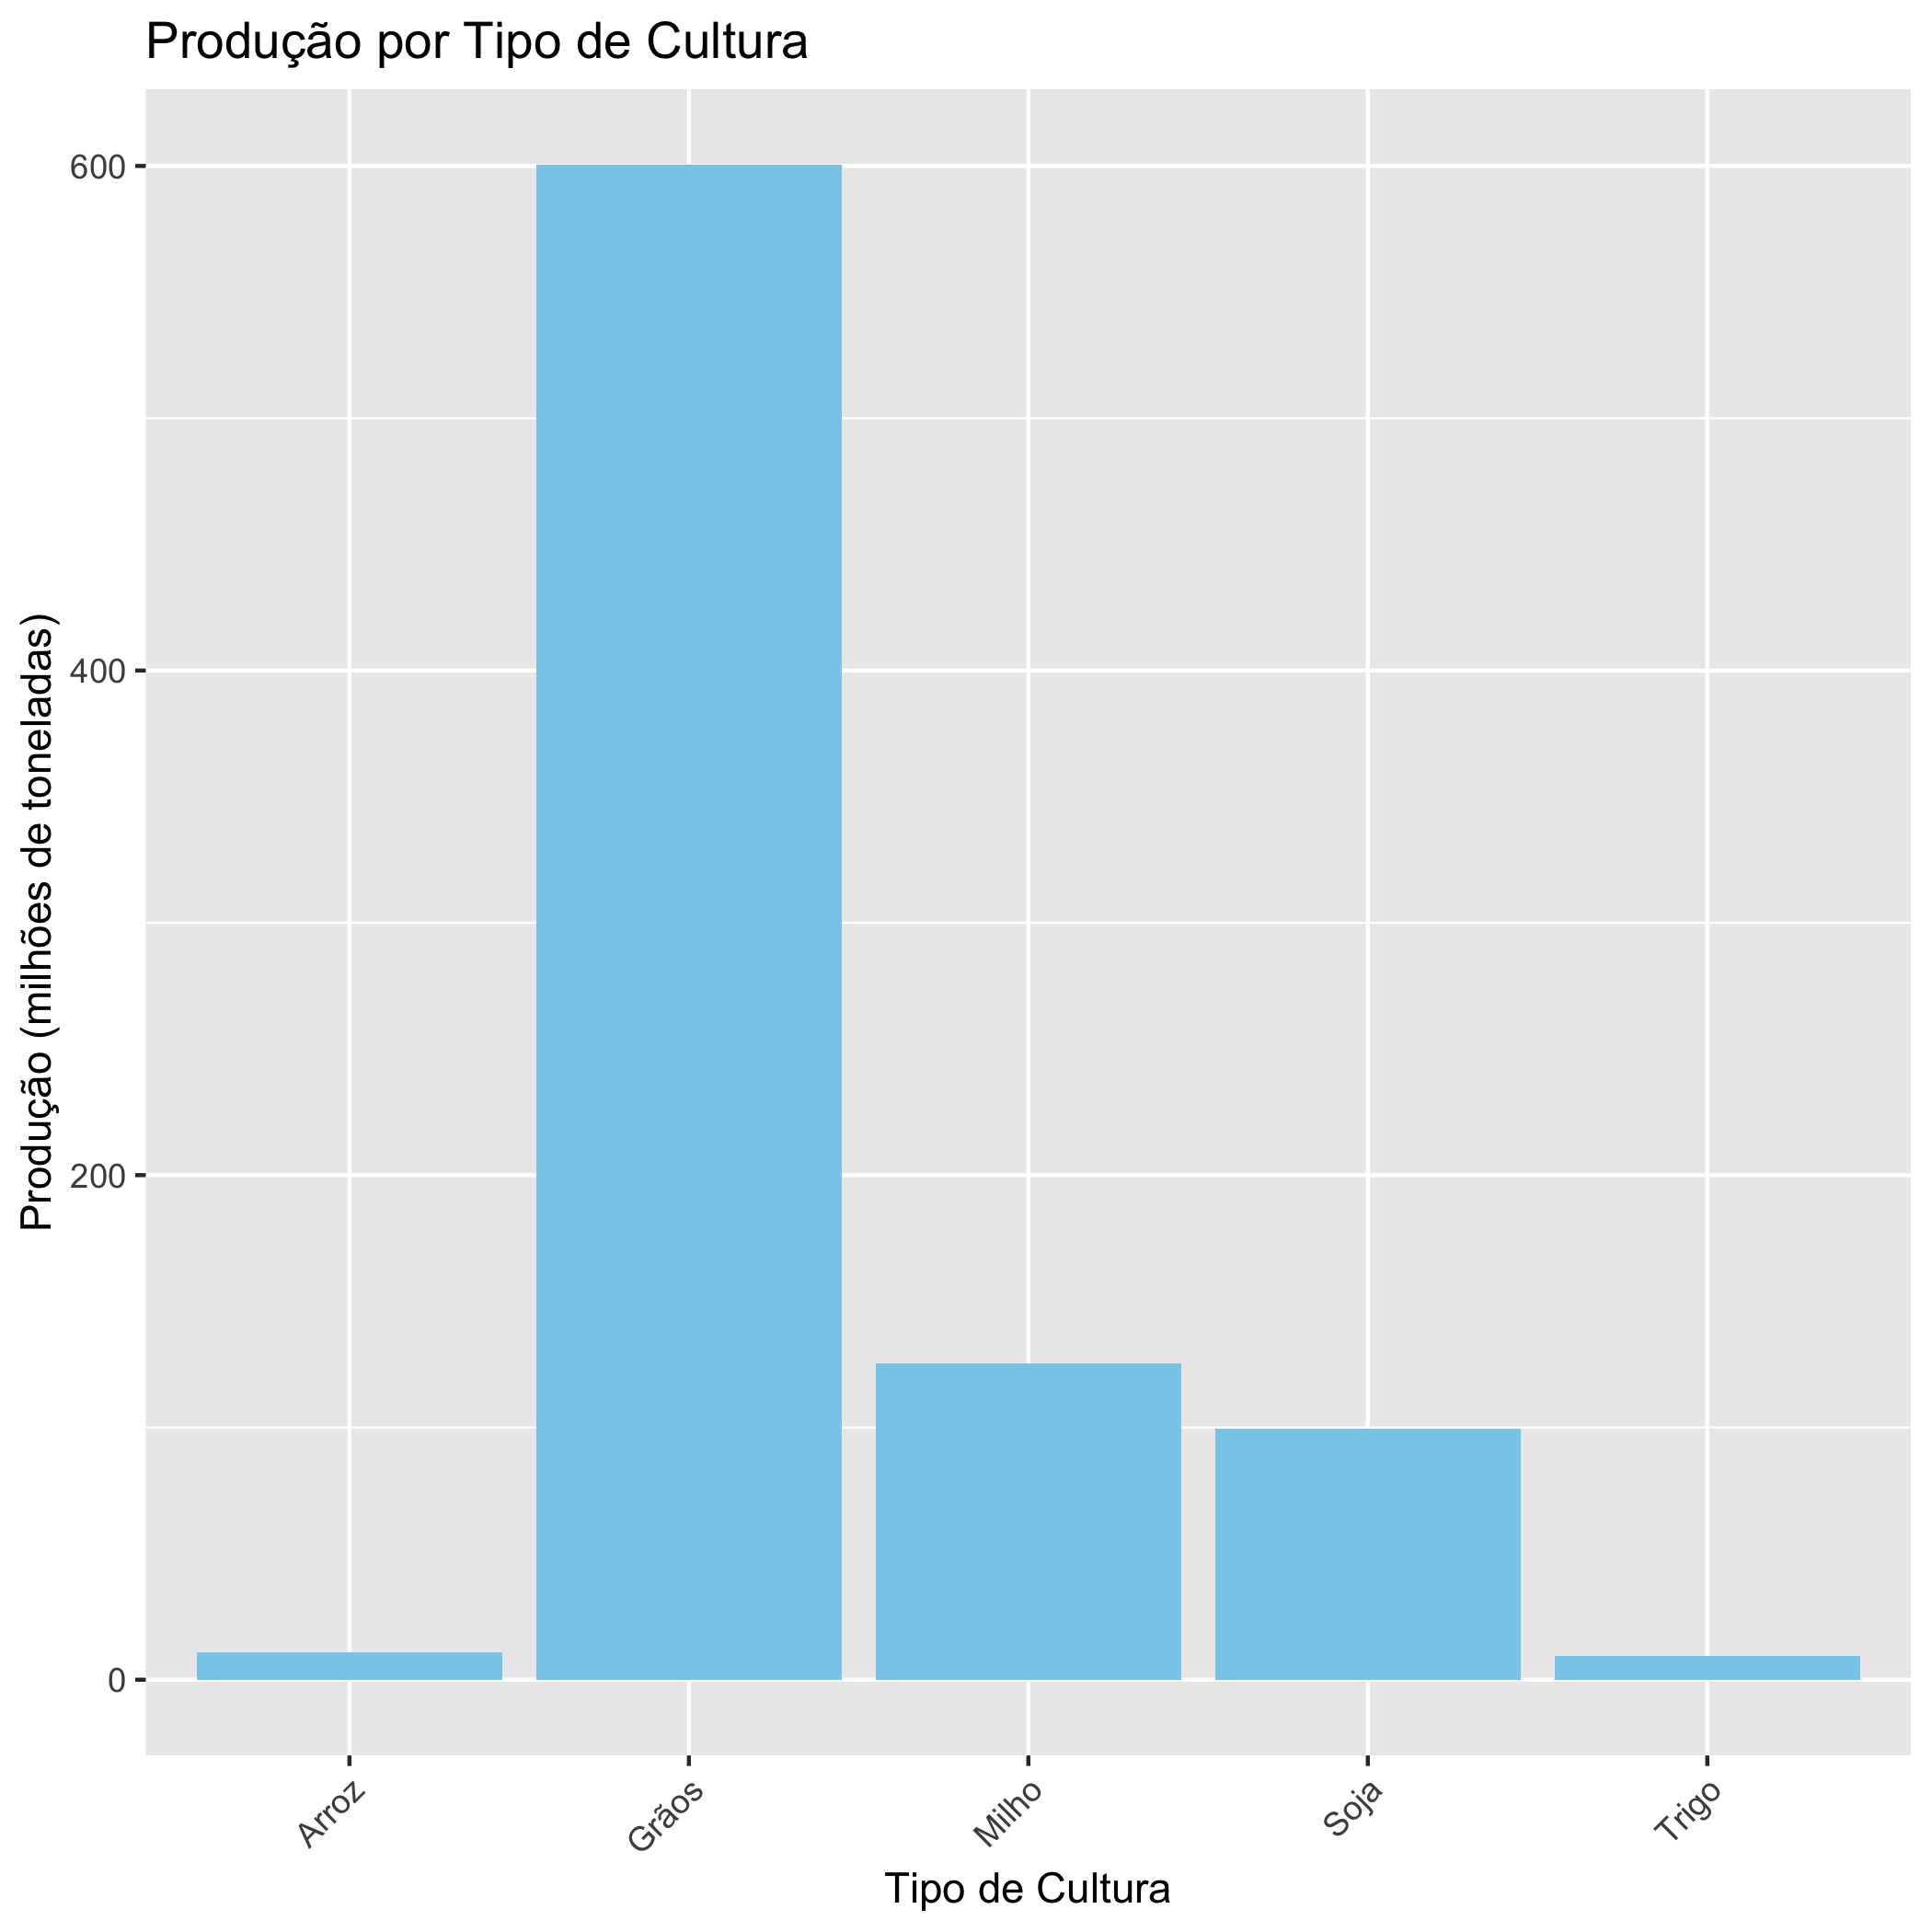
\includegraphics[width=\textwidth]{build/producao_por_cultura.png}

\section{Rebanho}
A análise do rebanho indica diferentes tipos e quantidades de animais na pecuária brasileira.

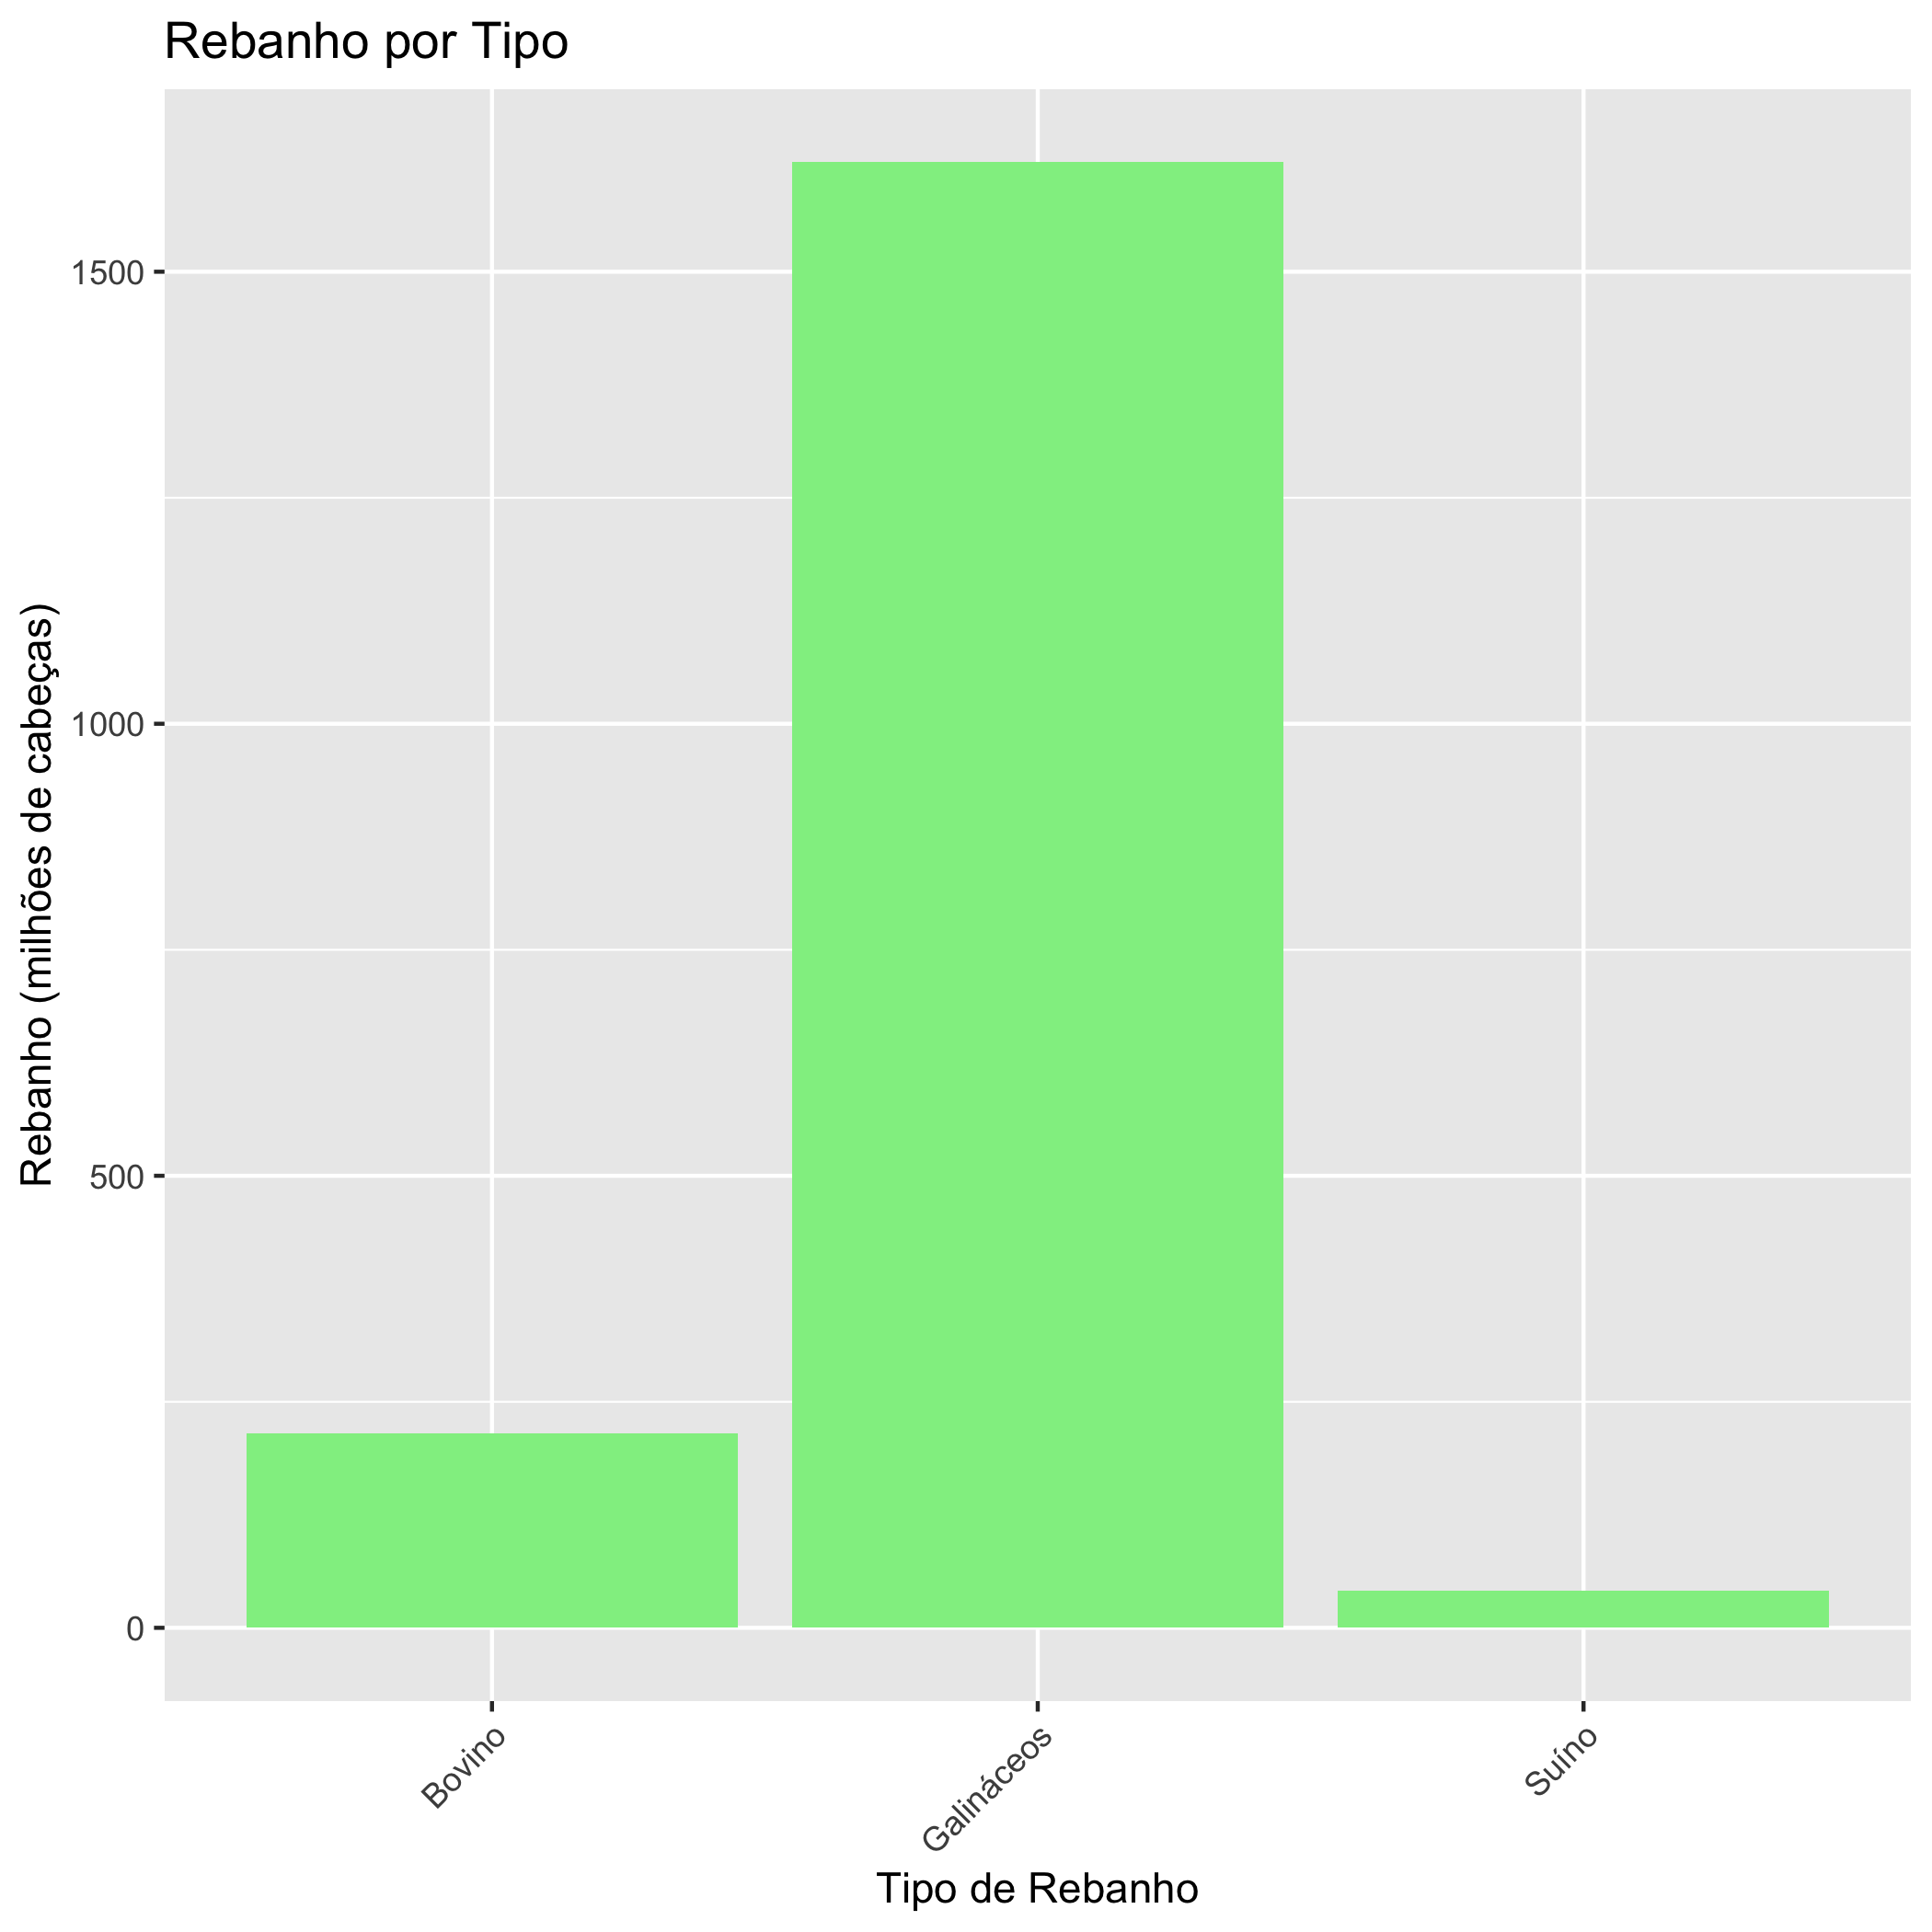
\includegraphics[width=\textwidth]{build/rebanho_por_tipo.png}

\section{Financiamento Agrícola}
Os dados de financiamento mostram diferentes tipos e valores de financiamento no setor agrícola.

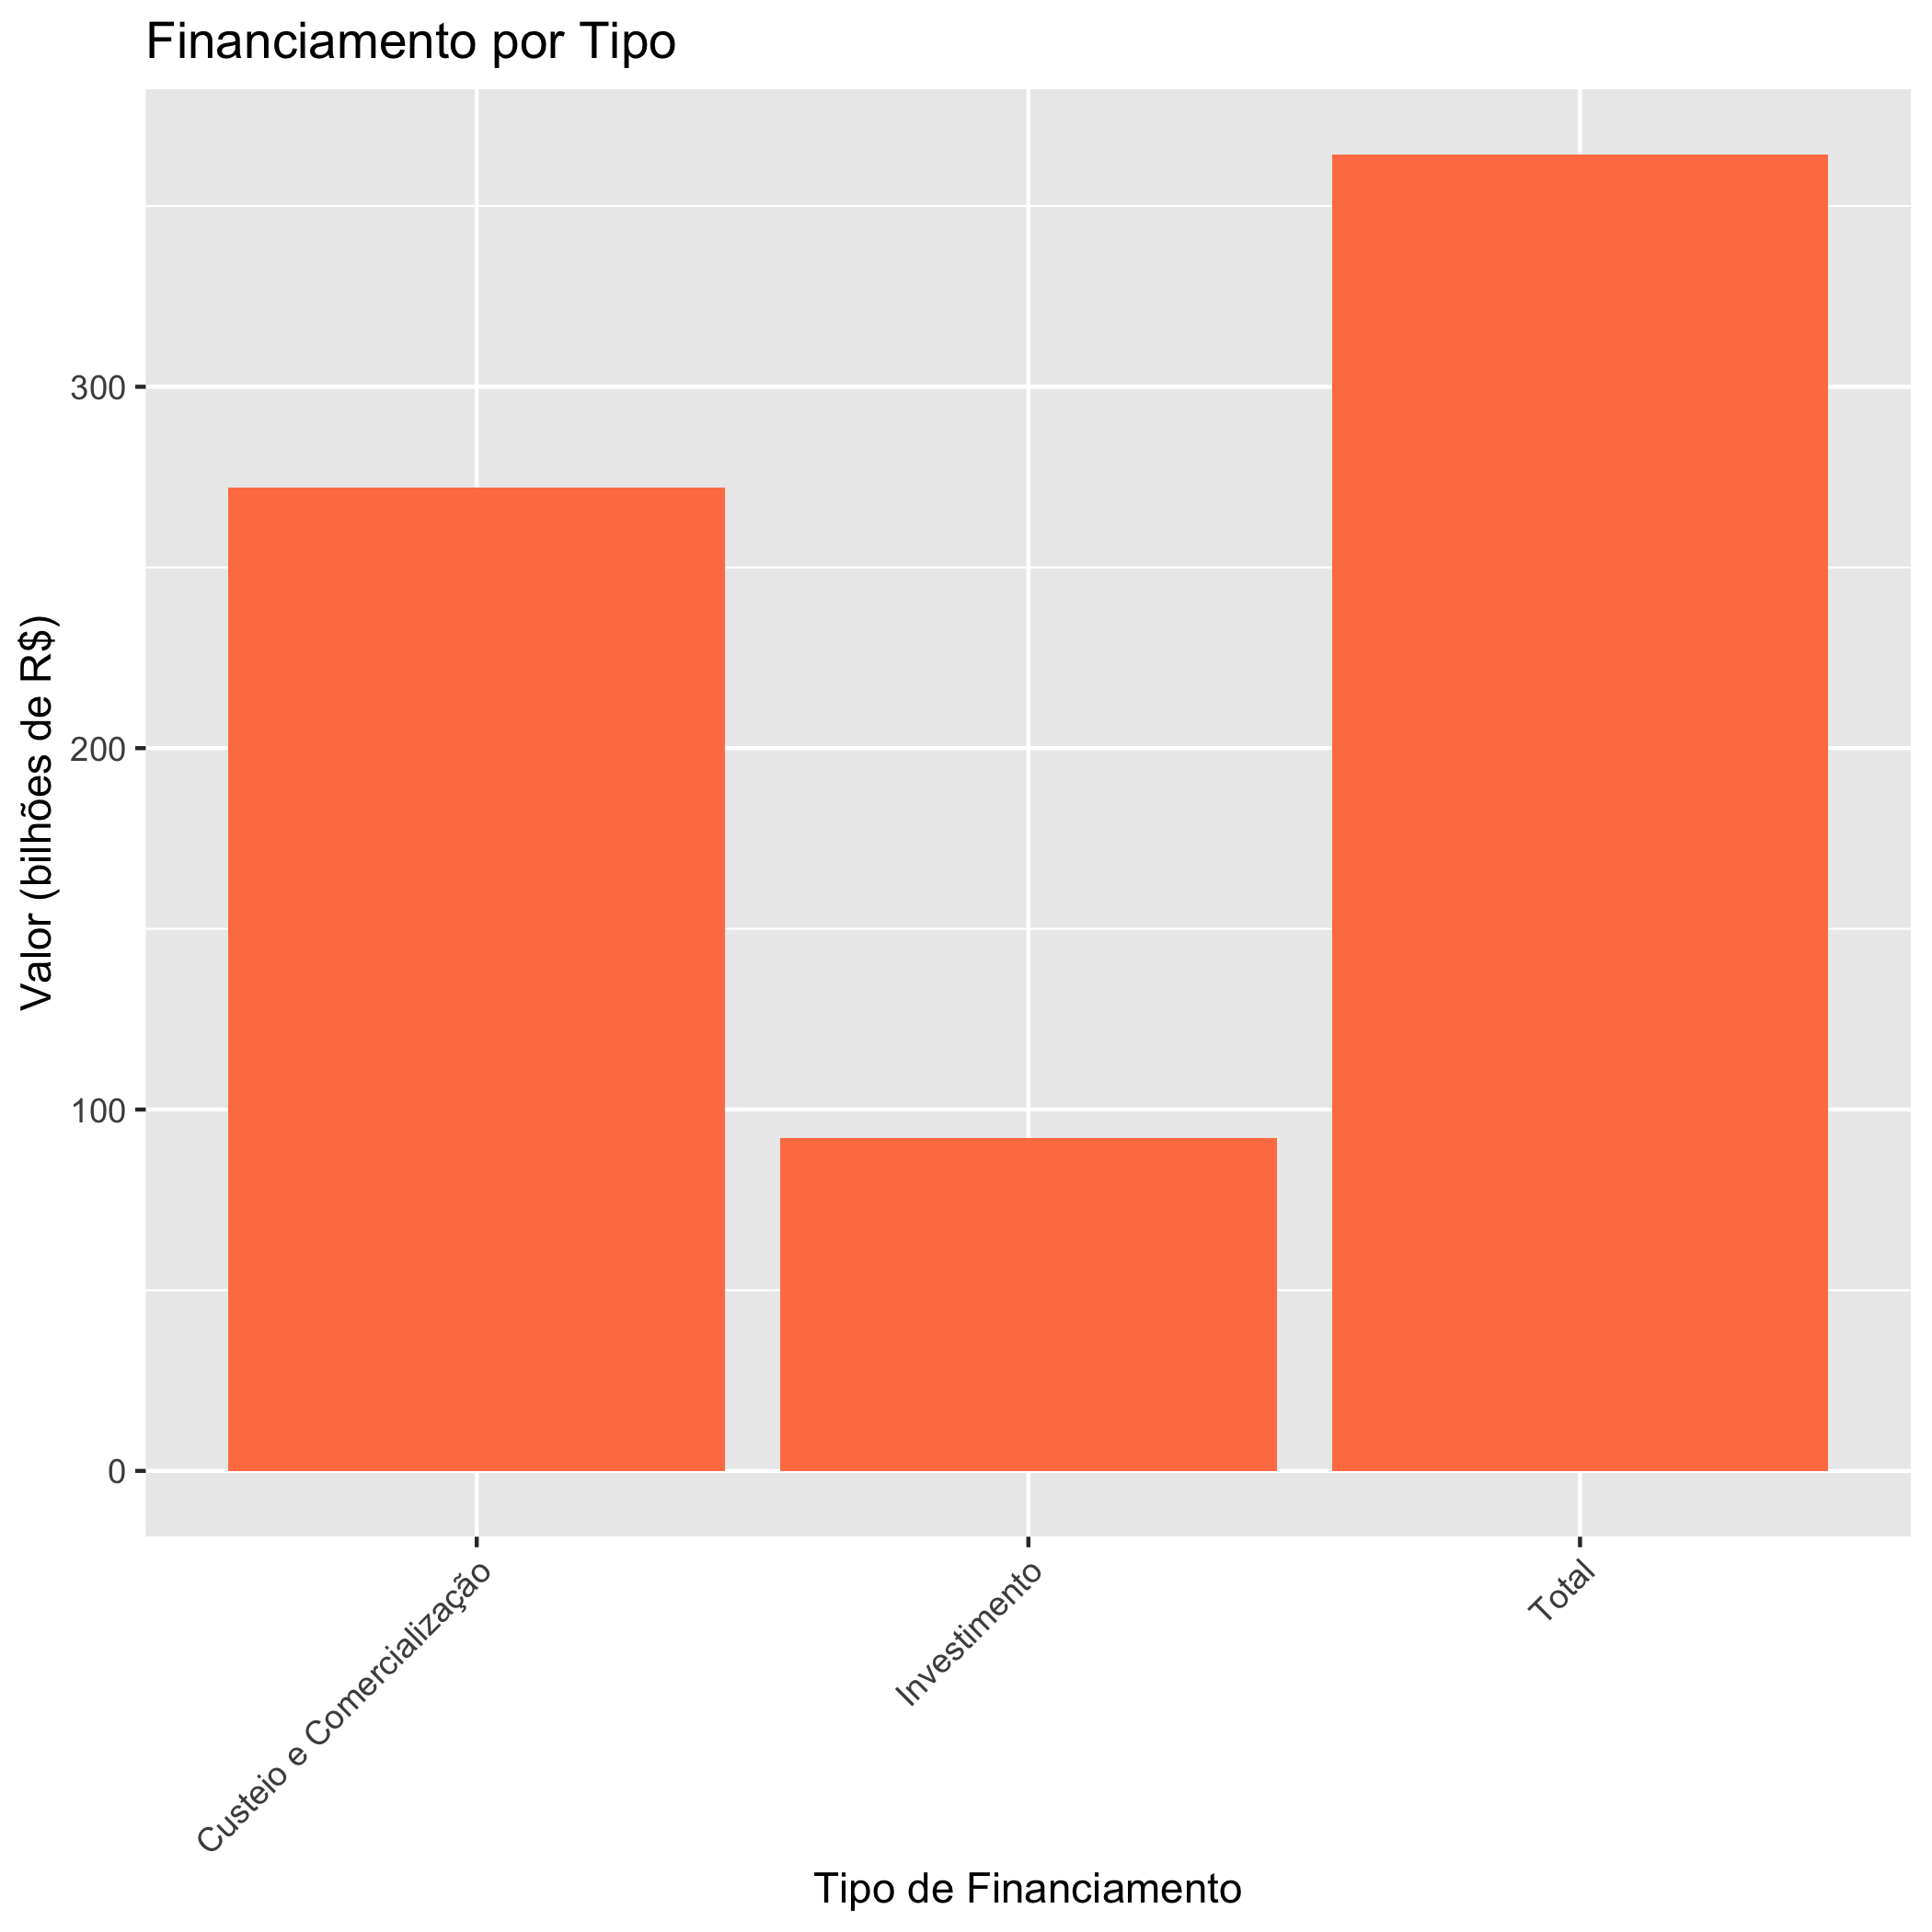
\includegraphics[width=\textwidth]{build/financiamento_por_tipo.png}

\section{Economia do Agronegócio}
A análise dos dados econômicos revela o desempenho do agronegócio ao longo dos anos.

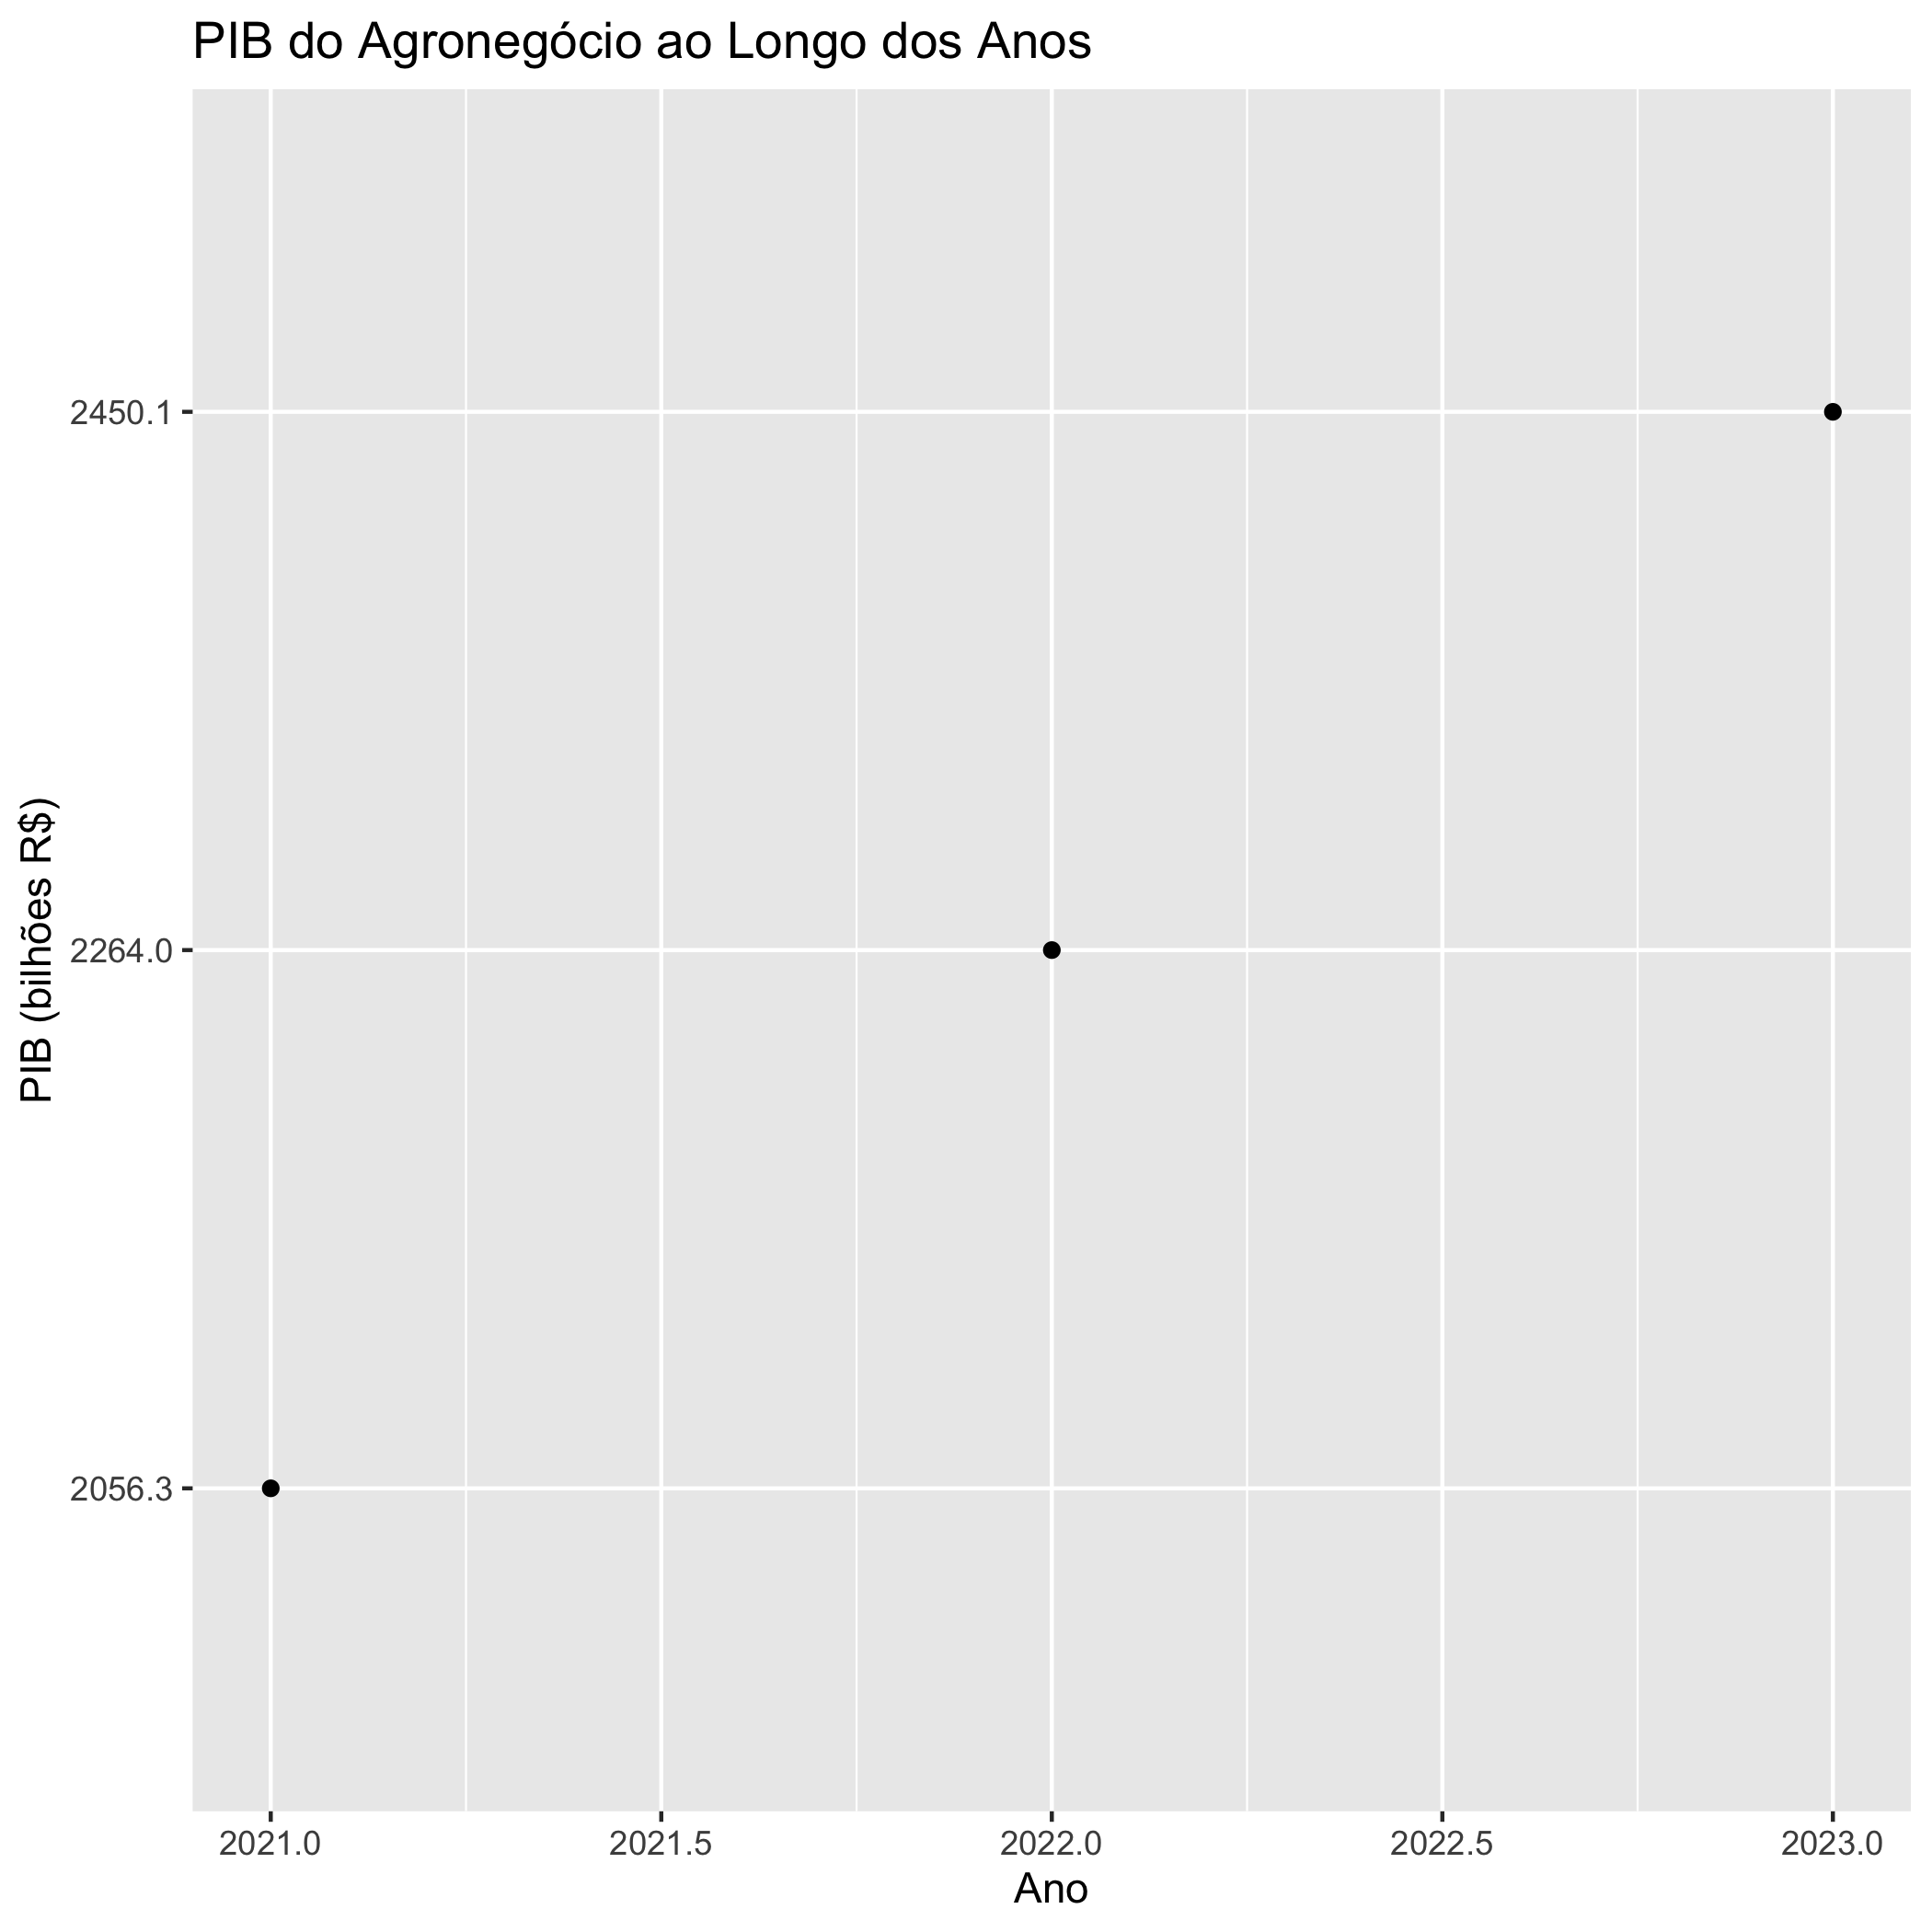
\includegraphics[width=\textwidth]{build/pib_agronegocio.png}

\section{Conclusão}
Este relatório fornece uma visão geral do agronegócio brasileiro, destacando tendências importantes e áreas que merecem atenção para o desenvolvimento sustentável do setor.

\end{document}
